% vim: set tw=78 sts=2 sw=2 ts=8 aw et ai:
\documentclass[conference]{IEEEtran}

\usepackage{ucs}
\usepackage{url}
\usepackage[utf8x]{inputenc}
\usepackage[english]{babel}
%\usepackage{hyperref}	  % use \url{http://$URL} or \href{http://$URL}{Name}
\usepackage{underscore}	  % underscores need not be escaped
\usepackage{subfigure}
\usepackage{verbatim}
\usepackage{float}
\usepackage{amsmath, amsthm, amssymb}
\usepackage{parskip}
\usepackage{flushend}

% Support for including graphics
\usepackage{graphicx}
\DeclareGraphicsExtensions{.pdf,.png,.jpg}

\begin{document}

\title{Mobile Gateway for Wireless Sensor Networks utilizing drones}

\author{
\IEEEauthorblockN{Ioan Deaconu, Andrei Voinescu}
\IEEEauthorblockA{
  Automatic Control and Computers Faculty\\
  University Politehnica of Bucharest,\\
  \{ioan.deaconu@cti.pub.ro, andrei.voinescu@cs.pub.ro\}}
  }


\maketitle

\begin{abstract}
% ********** Abstract **********
\chapter*{Abstract}

This thesis proposes a new way of implementing a mobile gateway for Wireless Sensor Networks that simplifies applications running in remote locations, where maintenance is difficult. Wireless Sensor Networks islands need a gateway connection in order to reach the outside world, but this is difficult to provide in all instances.  The solution to this problem is to use a gateway mounted on a UAV that can reach those islands and extract data from them. This has been proven to be feasible but adoption is low because of the high cost and the technical background needed to operate it. We propose a simpler, easier to operate and cheaper solution for this problem.




\textbf{Keywords} Wireless Sensor Networks, sparrow, energy harvesting, scheduling

\chapter*{Acknowledgements}

Foremost, I would like to express my gratitude to my advisor Dan Tudose for the continuous support that he provided.

Besides my advisor, I would also like to give special thanks to Dan Dragomir for providing corrections to this work.

My sincere thanks also goes to Adriana Drăghici, Alexandru Corneliu Olteanu and Dan Ștefan Tudose for their insightful comments  and moral support.

I thank my fellow labmates from Robolab robotics group: Tudor Vișan, Andrei Mușat and Andrei Vasiliu for the sleepless nights we were working together before deadlines, and for all the fun we had in the past four years.

Last but not the least, I would like to thank my family who have shown understanding and have given me the moral support needed.

% ********** End of Abstract **********

\end{abstract}

\begin{IEEEkeywords}
gateway, wireless sensor networks, drone
\end{IEEEkeywords}

\section{Introduction}
\label{sec:introduction}
\normalfont\normalsize
\chapter{Introduction}


A big problem encountered when developing an application for  Wireless Sensor Networks is autonomy.
Big batteries can be used to power the nodes, but because some can be deployed in locations
difficult to reach, a simple task of changing the batteries becomes an impossible one.

The solution to this problem is powering the devices from alternative sources of energy, a process
called energy harvesting. In recent years, energy harvesting has become more and more used in the field of Wireless
Sensor Networks. There are plenty of alternative energy sources, such as solar cells, vibration
absorption generators, wind mills, thermoelectric generators and others, that can be used to power the
nodes or charge their batteries in order to become autonomous.

While the energy source problem has a solution, another problem appears in the form of finding a
method to store the generated energy. A battery could be used to store the generate energy, but
unfortunately, current technology allows to charge one for a few hundreds of cycles.
Considering that a cycle would be used per day, in maximum 2 years, the battery will lose most of
its original capacity. An alternative to the battery is using a super capacitor, which has a
lifetime of 10 years or 500.000 cycles, but are more expensive and store far less energy than regular
rechargeable batteries.

In order to alleviate the problem of the small amount of stored energy, a scheduling algorithm can
be used. The main goal of the algorithm is keep the functional between two sessions of generated
energy without losing power and to send as much data as possible. This is achieved by dynamically
varying the frequency with which the node performs various tasks or sends data.

In this thesis we will describe the architecture of an energy harvesting wireless sensor network
(EHWSN). We will present a new node and development platform, the Sparrow R, designed
for low power and the problems we encountered when creating a EHWSN application. As the final part
of the architecture, we developed an efficient but lightweight algorithm for efficiently using the stored energy.




\section{Related Work}
\label{sec:related}
Nodes for wireless sensor networks have been created in the past \cite{voinescu2013lightweight}, V3.2 is a successful
iteration based on Atmel Atmega128RFA1. Paired with the node, a dongle can be connected to a
computer using an USB port which allows the PC to act as a gateway for the network of nodes. Even
though the node is very low power, developing new applications on the node is very complicated. The
only way to program a node is using an ISP programmer using a dautgher board that contains a JTAG
and ISP connector and a FTDI for usb to serial connection. Adding new hardware is very difficult, the expansion
capabilities are limited which leads to using only the existing sensors mounted on the node.

\begin{figure}[ht] \centering
\includegraphics[width=0.5\textwidth]{img/sparrowv32.jpg}
\caption{Sparrow V3.2 with gateway and programming base board}
\end{figure}


The next iteration, the Sparrow V4 based on the same microcontroller as Sparrow V3.2, tried to fix
the development environment by being Arduino \cite{arduino}
compatible. This removed ISP programming, but it is still necessary to use the extensions daughter board
with FTDI in order to program the board. The limited expansion capabilities are still an issue and, unfortunately, the node
has a very high power consumption of between 400uA up to 1.5mA \cite{geo} when in deep sleep.

Another problem is that Sparrow is directly powered from an external source, which we must make
sure it is between 1v8 and 3v6, depending on the sensors maximum operating voltage, otherwise there
is a possibility that some components might be destroyed. Because the
microcontroller has an internal LDO, it will have the same current consumption regardless of the
operating voltage resulting in the power consumption to vary between 7.4mW up to 14.8mW for the cpu
and between 32.5mW up to 65mW when transmitting data. Also, the power for on-board sensors is cut
using an mosfet-N on the common GND line. Due to this, some sensors can "borrow" the GND from
digital pins which increases the power consumption.
\begin{figure}[ht] \centering
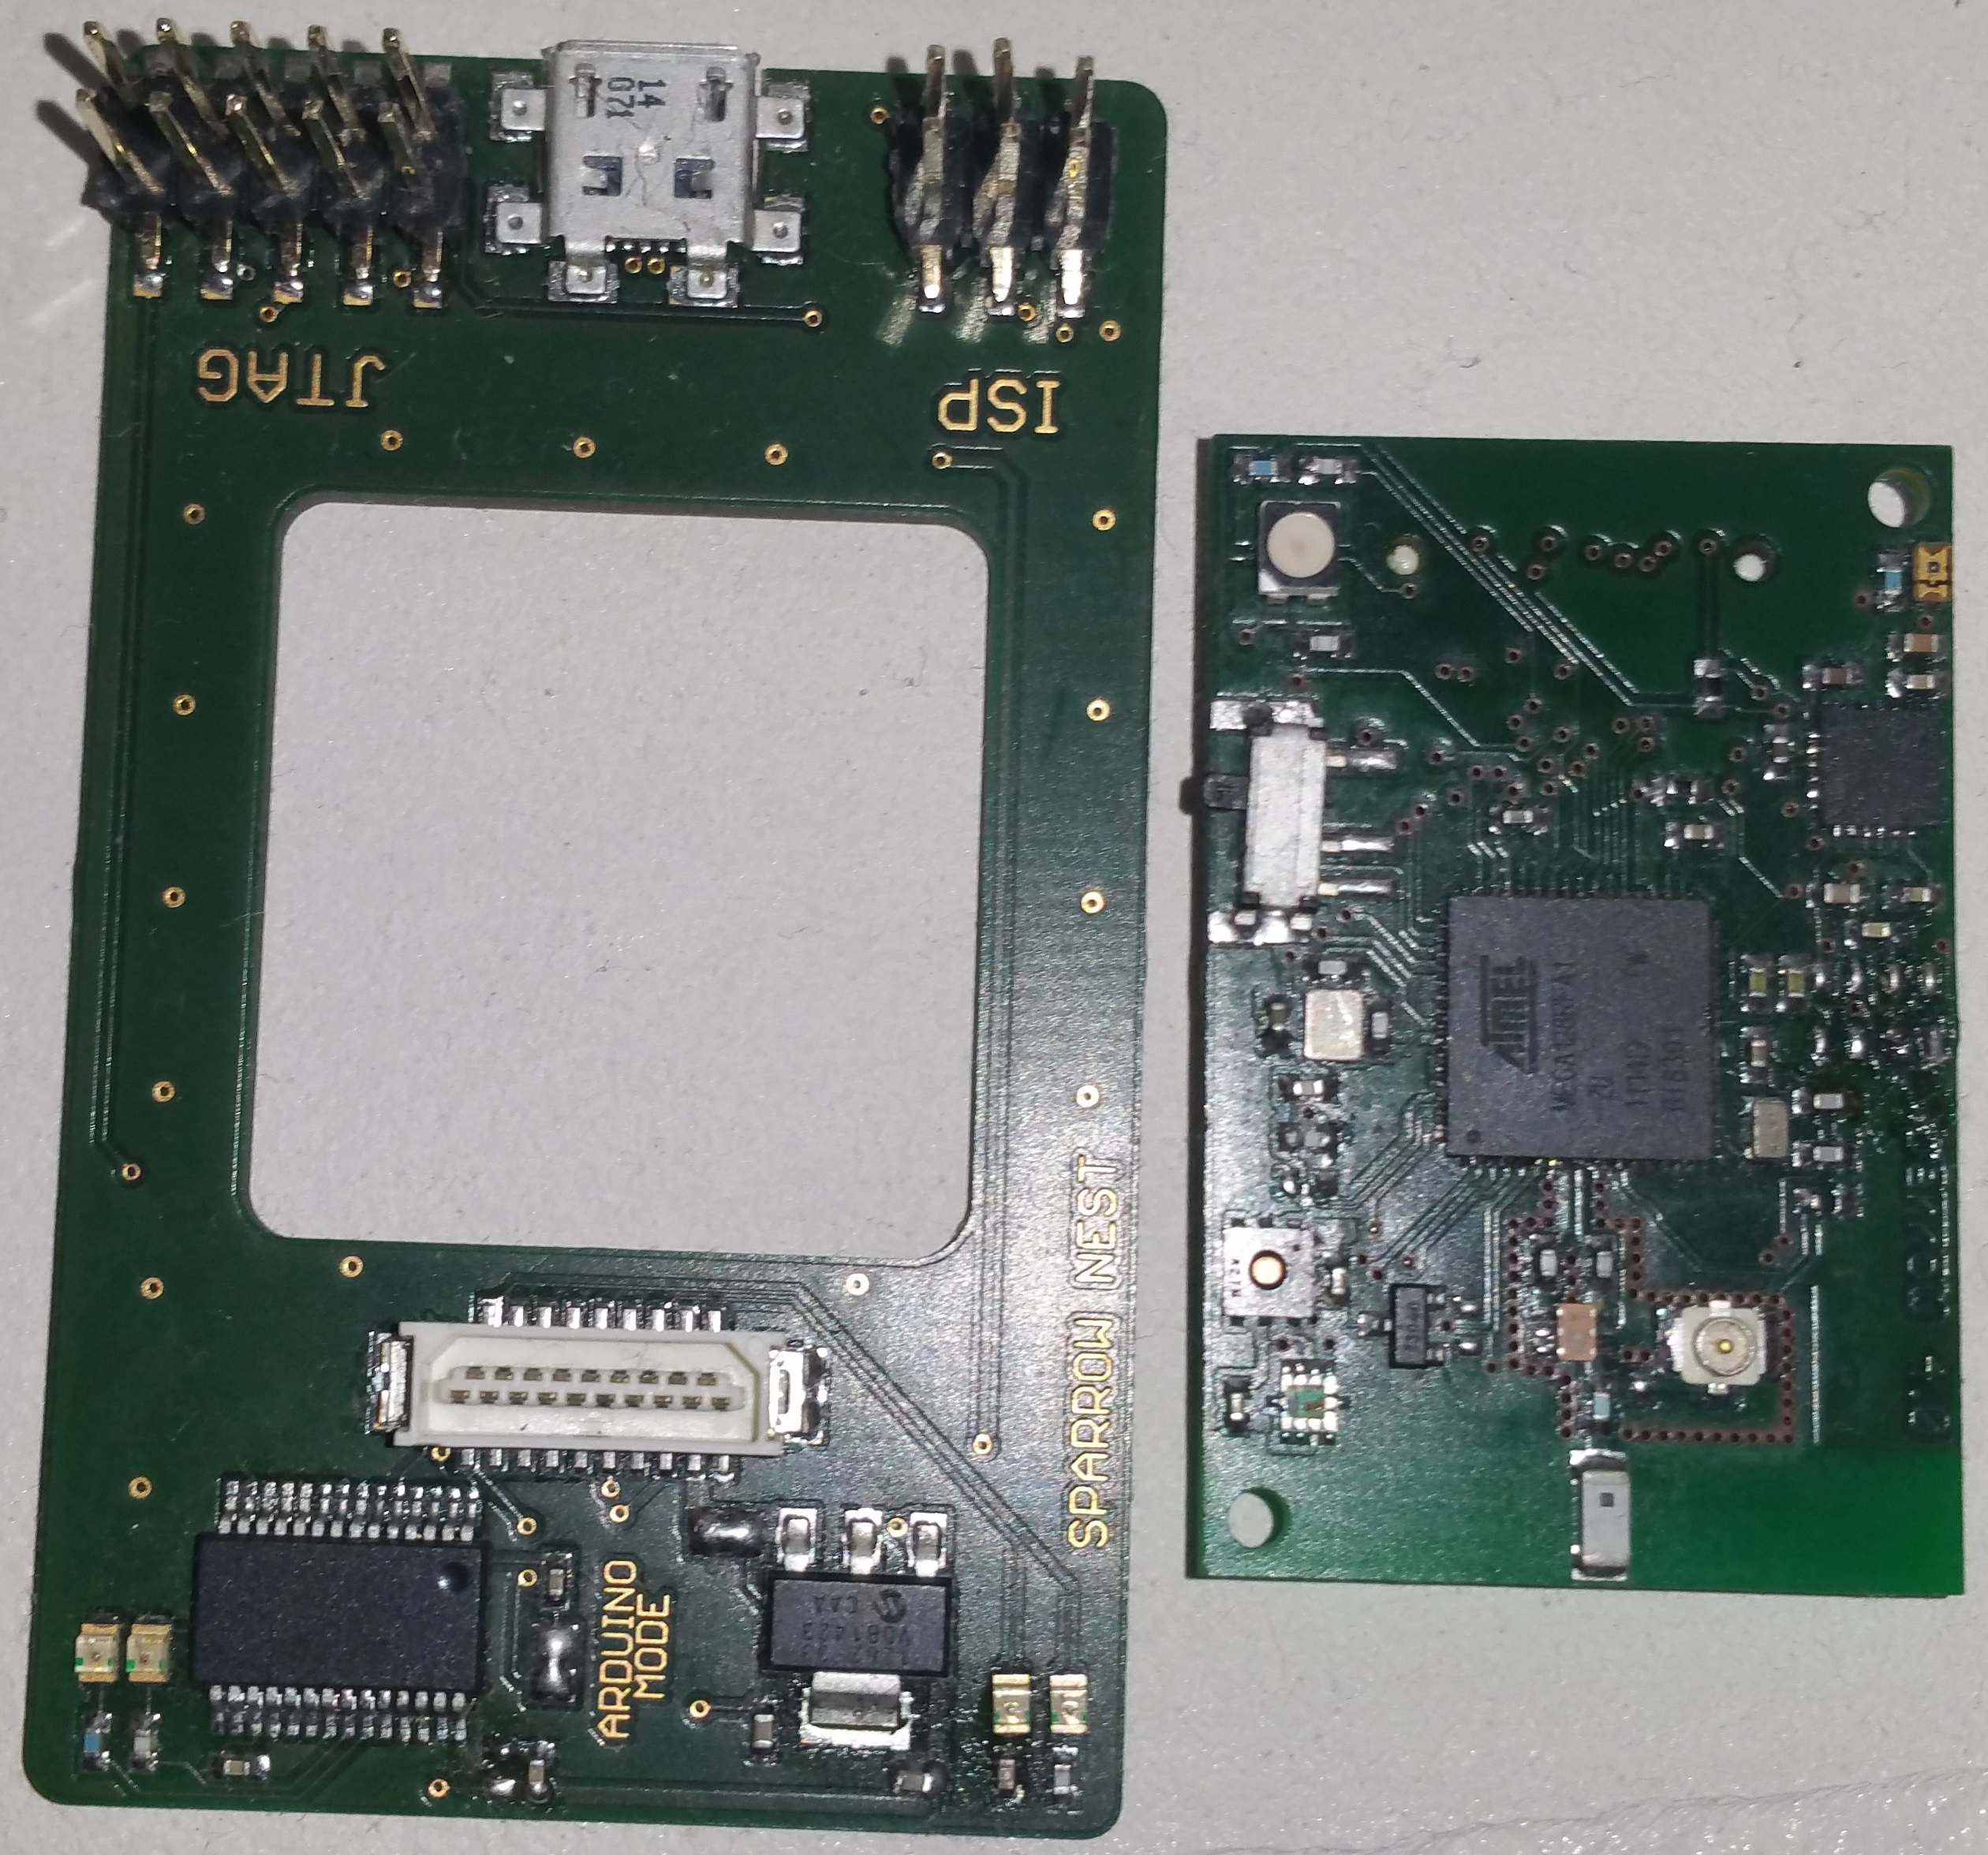
\includegraphics[width=0.5\textwidth]{img/sparrowv4.jpg}
\caption{Sparrow V4 with programming base board}
\end{figure}





\section{System architecture}
\label{sec:architecture}
\label{chap:arch}

\subsection{\textit{Hardware}}
Because not all sensors are designed to run at 1v8 up to 3v3, we need to be able to dynamically
change the operating voltage of the node. We used TPS62742, a step-down switching DC/DC converter
with up to 90\% efficiency, voltage selectable output from 1v8 to 3v2 with 200mV step, 360nA
quiescent current and a special mcu controllable load output, with push-pull transistors. In
inactive state the load line is pulled to GND and when active is pulled to VCC. When active it
consumes 12uA, but compared to the controlled sensors, this should not be noticeable. Because this
allows to completely power down the sensors, the "stand-by" current consumption is 0uA and it also
eliminates the previous design problem of floating GND which allowed the sensors to "steal" power
from other pins and not be properly disabled.

The node can be connected to an extension daughter board which fully respects the Arduino pinout.
The advantage of this approach is that it allows to easily test and prototype new configurations in
order to be prepare the project in the shortest time possible. Also existing hardware designed for Arduino can work with this board,
which increased the number of compatible hardware. In total, 20 I/O pins are available, pins that
can be used for connecting sensors, either on the daughter board, or directly on a specialty
designed board.

A jumper can select whether the Node is powered from USB or from other 2v1+ voltage supply. Through
the same jumper a power measuring device can be used to monitor the total power consumption. In case the DC/DC converter is not
needed the node can use other power source.

\subsection{\textit{Performance}}

The SAMR21\cite{samr21} micro-controller is an ARM cortex M0+ core clocked at 48 MHz with 32KB of RAM and 256KB
of flash. Being a 32-bit architecture and a new architecture, even though SAMR21 consumes 5.5mA
compared to 4.1mA of Atmega128RFA1, for simple 32-bit integer addition, SAMR21 consumes only 49nJ
per iteration while the 8-bit micro-controller consumes 274nJ, almost 5 times more. Considering
performance figures, SAMR21 was 9 times faster with 403950 iterations per second while
Atmega128RFA1 managed only 44890 iterations.

Testing the performance of branch predictor, revealed that the M0+ is only 12\% better than
the older 8-bit counterpart, but thanks to the frequency difference, it ends up being 3,36 times
faster.


\begin{figure}[ht] \centering
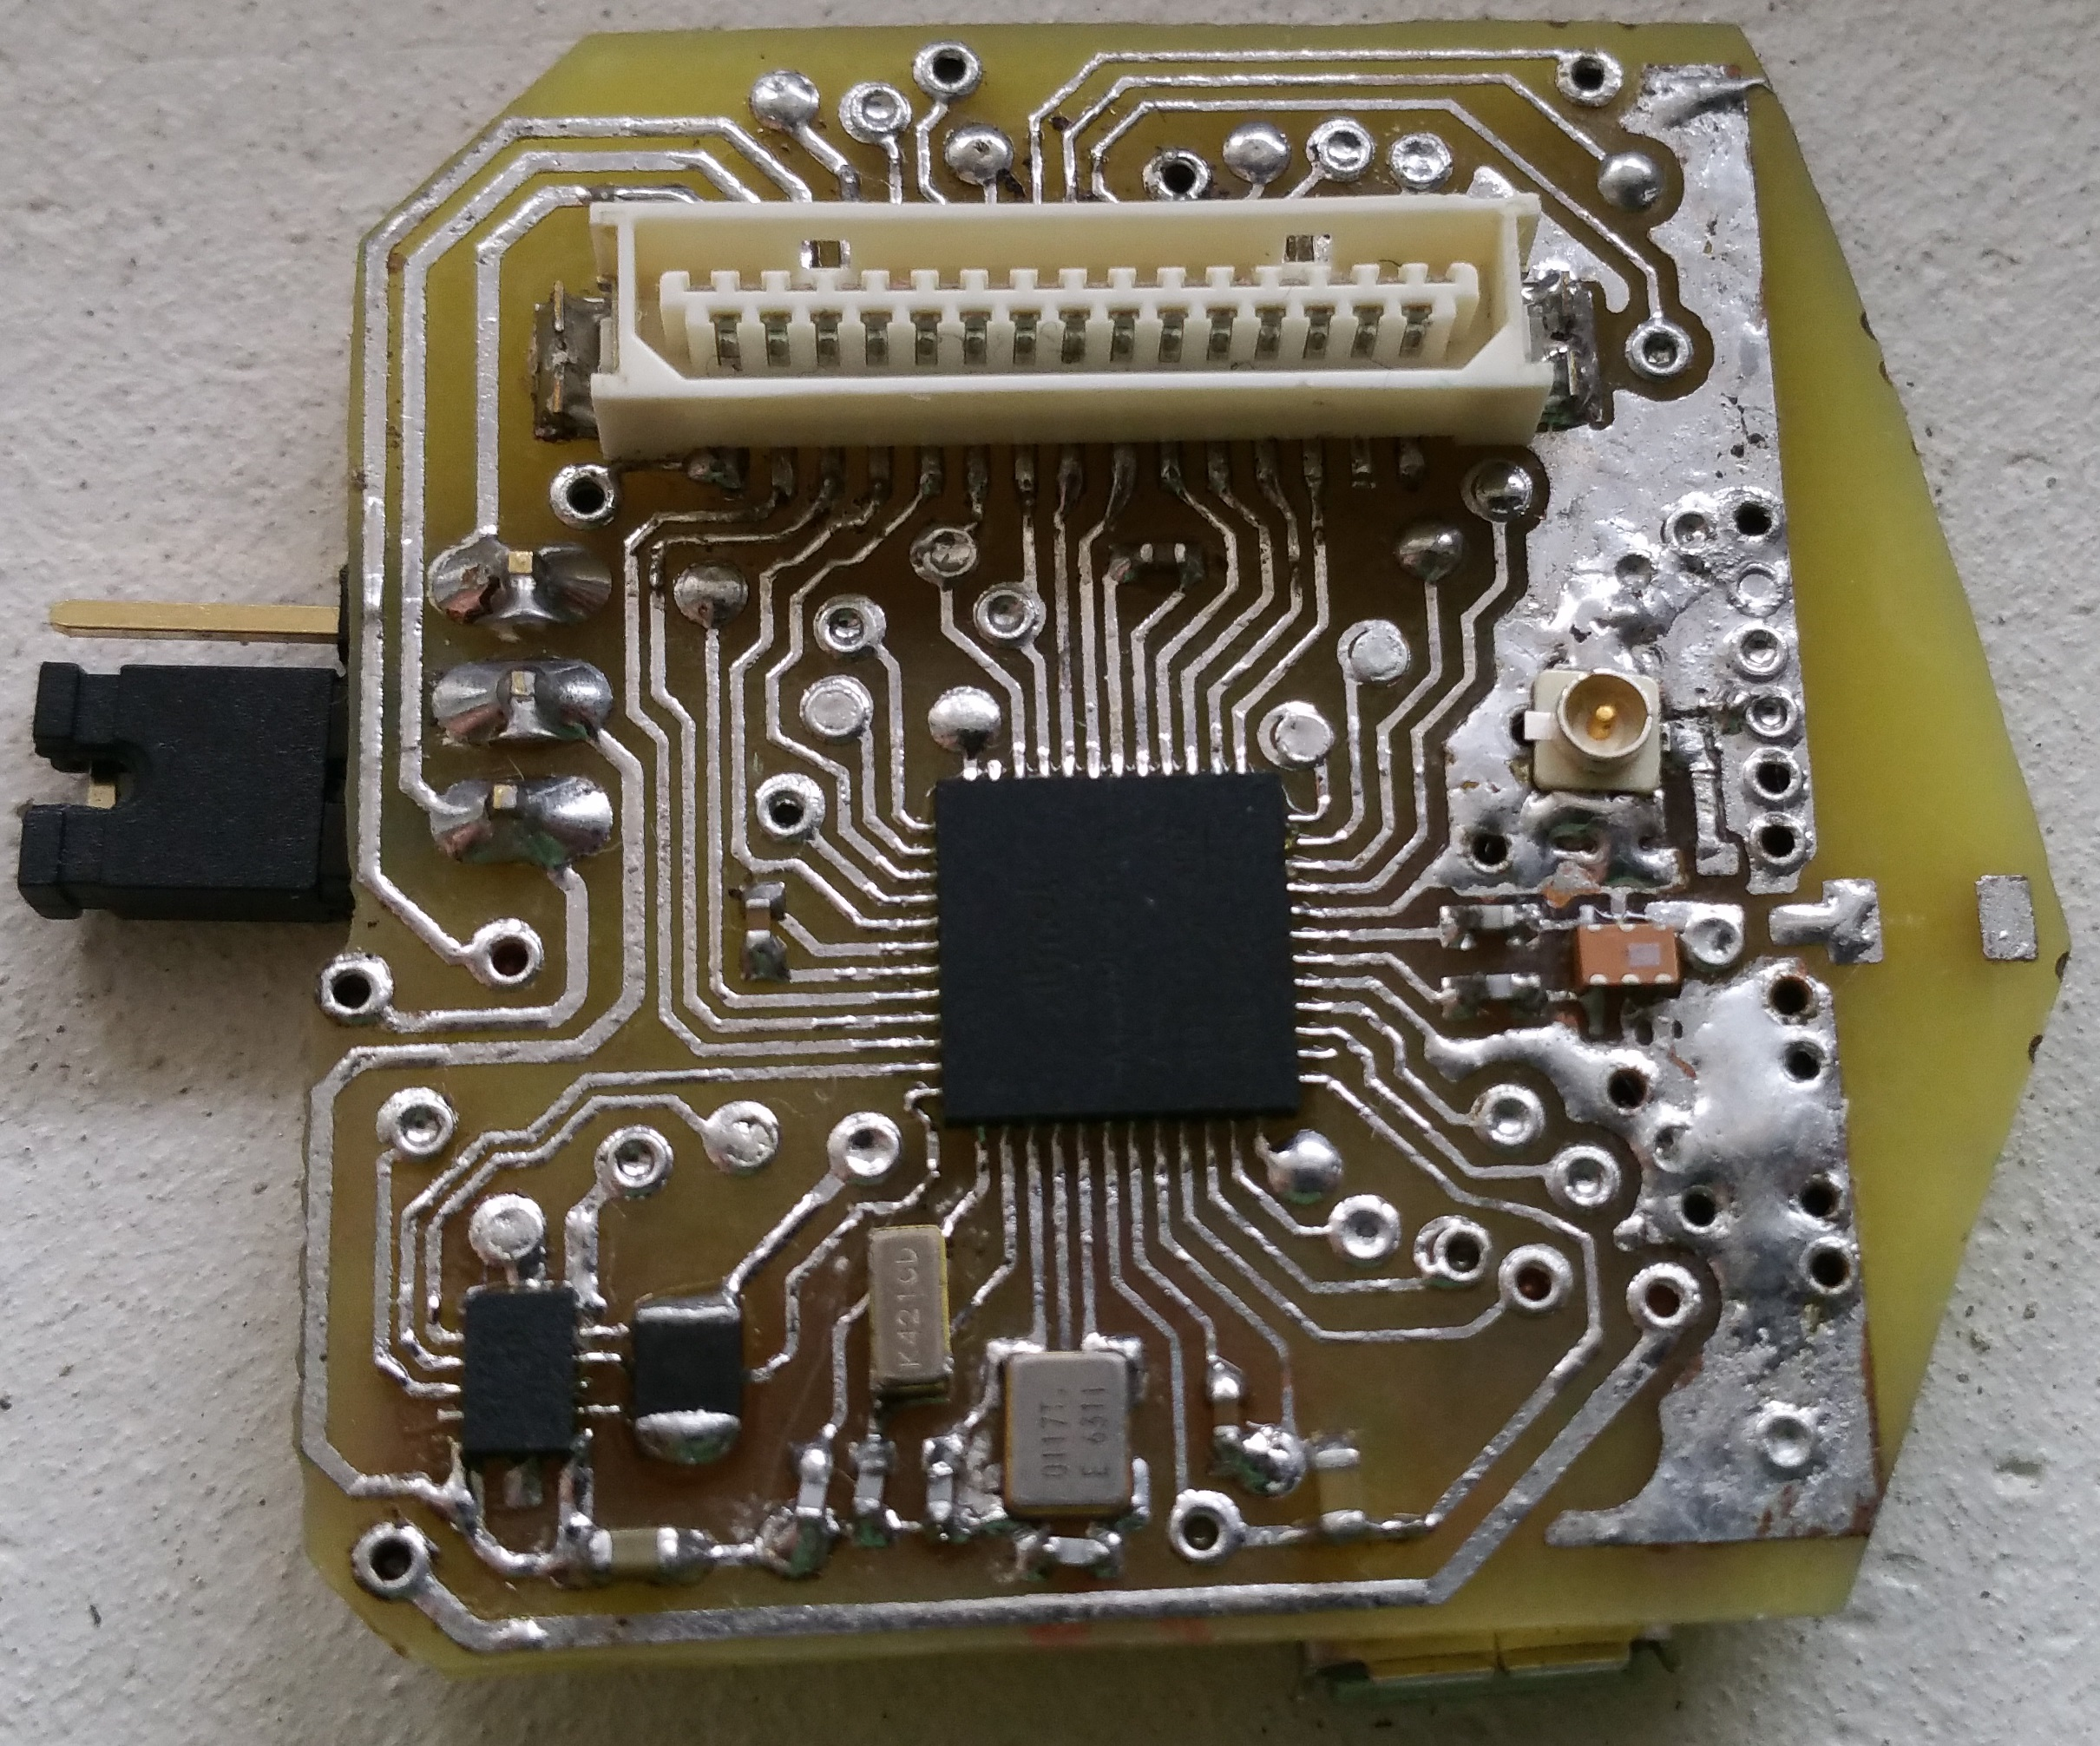
\includegraphics[width=0.5\textwidth]{img/sparrowrf.jpg}
\caption{Sparrow R node}
\end{figure}

The SAMR21 micro-controller is almost the same micro-controller as SAMD21 \cite{samd21}, which is used in Arduino
Zero boards. This allowed use to use exiting code, but unfortunately a not well
written one.

Even thought the Arduino software is well designed, it was not designed with low power approach
from the beginning. We will describe some of the problems encountered when trying to create the software stack.

The first problem noticed was that the Arduino Zero board had no sleep functionality implemented.
The ideal idle current consumption should have been less than 5uA, tested and measured using a
project created in Atmel Studio 7.0. The current consumption of the board was around 350uA. Further
tests revealed that the USB device was always initialized, which accounted for the extra 200
uA. The rest of 150uA came from a default initializations of the pins as input pins, but this only
lowered the current consumption to about 60uA. We kept searching for a cause, and discovered that
the clock generators are never disabled at start-up, which accounted for about 30uA.

So far we managed to decrease the idle current consumption for the platform from 350uA to about
30uA @ 3v2, but it is still far from ideal. Surprisingly, lowering the voltage from 3v2 to 1v8 lead
to  decrease in sleep current consumption down to 3.3uA. When examining the power trace using a digital oscilloscope, we found
that a very low frequency clock remains active, which at 3v2 has high spikes in power consumption.

Tough we did not reach the goal of 5uA, we still managed a respectable 30uA @ 3v2 and less than 4 uA @1v8.
Due to the time constrains and the need to use the nodes in order to implement and test new
features, we decided that for now this is acceptable, and for future revisions, we will come back
and find the extra clock source.

Even the run current consumption was not ideal, instead of achieving the promised 70uA/MHz @ 3v2,
or around 3.5mA @ 48MHz, the micro-controller consumed 8mA @ 48MHz. We managed to reduce the current consumption to 5.5mA @ 48MHz, due to
clock optimizations presented bellow.

The first change was to change the clock of the peripheral interfaces, instead of 48 MHz, we run them at 12 MHz.
Also if peripherals are not used, we completely disable them. Due to this, we ran into problems
related to SERCOM implementation, a generic module that handle USART, SPI and I2C. It was working
on Arduino Zero, because the CPU and the BUS were configured to run the same speed, but due to the
previous clock source modifications, the SERCOM did not set the correct speed. Also, there are 6
SERCOMs, and instead of enabling the clock for each one only when it is used, all of them were
enabled, which lead to extra power consumption during run time.

\begin{figure}[ht] \centering
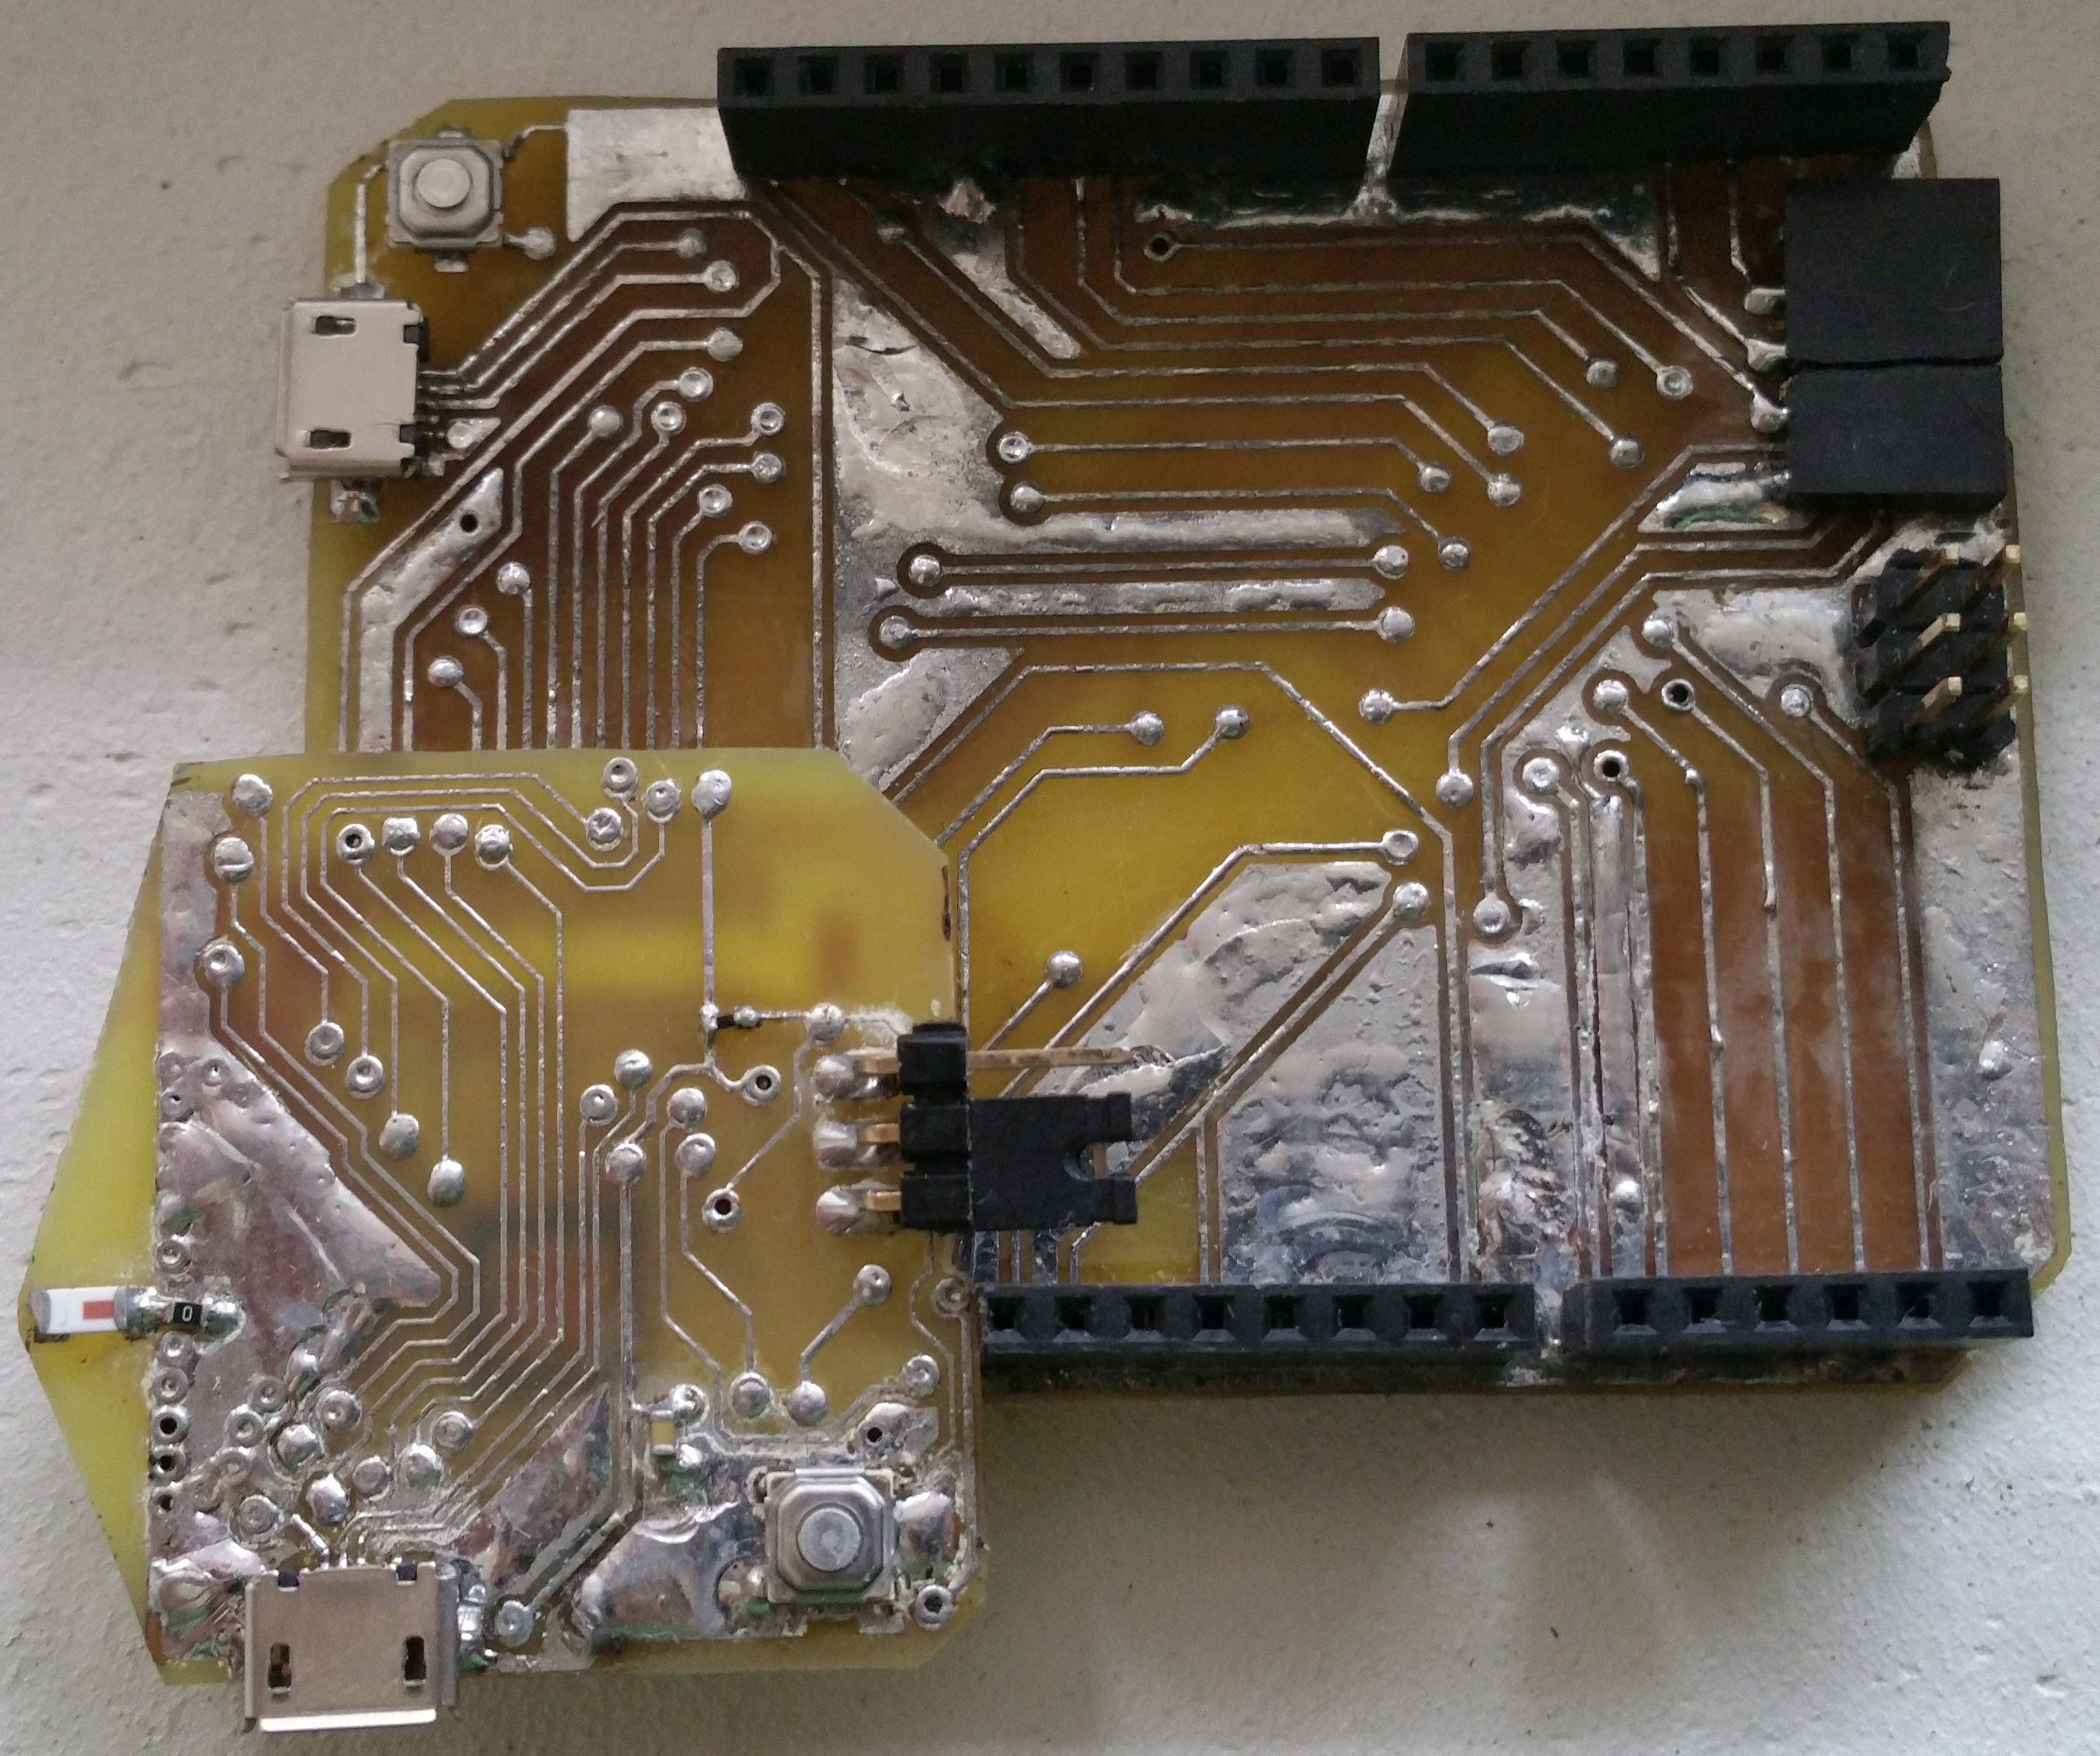
\includegraphics[width=0.5\textwidth]{img/base-with-sensor.jpg}
\caption{Sparrow R node mounted on Aduino compatible base}
\end{figure}
\subsection{\textit{Software}}


We implemented new modules designed for low power like sleep, power management which can dynamical
change the running voltage between 1v8 to 3v2 when requested and enable or disable the LOAD power
line. This allows the user to select which voltage is better required for applications. For example,
some sensor must be powered at exactly 2v8 while others at 2v5 or lower. This module allows for
precise voltage selection with 200mV increments, use the sensor and then switch to the lowest
voltage in order to obtain the best power consumption possible.

The RF module is AT86RF233, integrated into the micro-controller. An Arduino library
\cite{rf233}
exists for the RF but in order to add new features, we integrated the module for the RF in the core
of the platform. This allowed us to let the user focus on what to do with the platform and not how to do
something with it. Furthermore, extra futures and bug fixes are easier to be implemented if the module is
integrated in the platform. For example, in case the RF is constantly running in receive mode for
more than 5 minutes, it is recommended to do Fine Tuning of the PLL clock in order to eliminate
possible clock skews. Feature wise, when the module automatically receives a packet, it saves it
locally together with RSSI and LQI, which can be later read and used buy the user. The internal
buffer is designed for 8 packets of 127KB of data, which amounts for 1 KB of ram. The buffer is
cyclic, so in case the buffer is not read, the oldest data is discarded and replaced by a new one.
This should not happen very often, because the buffer is large enough to handle all request, even
for high bandwidth transfers.

If the user has a need to save the data in case of power failure, the micro-controller has an
EEPROM like functionality which allows a 16KB region of flash to emulate EEPROM write endurance.
The flash contains pages of 64 bytes, and the EEPROM has an overhead of 4 bytes, which leaves 60
bytes for actual data. Also, for each page, another page must be reserved for further use.
The results is that out of 16KB used, the total amount of usable space left is $\frac{16*1024}{2}
* \frac{60}{64} = 7680 bytes$. This should be more than enough for normal use because the normal
endurance of 25k cycles of flash write and erase are increased to at least 150k, with typical
values reaching 600k cycles. If a new software is uploaded, the EEPROM zone is completely erased.

For timekeeping when sleeping, RTC functionality was implemented. Besides keeping the time, RTC
provides alarm interrupts for a special date, which can be configured to be triggered every
minute, every hour, every day, every month, every year, or only once. Together with another
peripheral named EventSys, periodic interrupts are provided and the interrupts interval can range
from once every second up to 128 times per second, with increments of power base 2.

Because the software and hardware are never perfect, a watchdog functionality is also implemented,
in order to avoid code lock-up or hardware failure due to extreme environment conditions.



\section{Implementation}
\label{sec:implementation}
\label{chap:impl}

 \subsection{Hardware Details}

\begin{figure}[hb] \centering
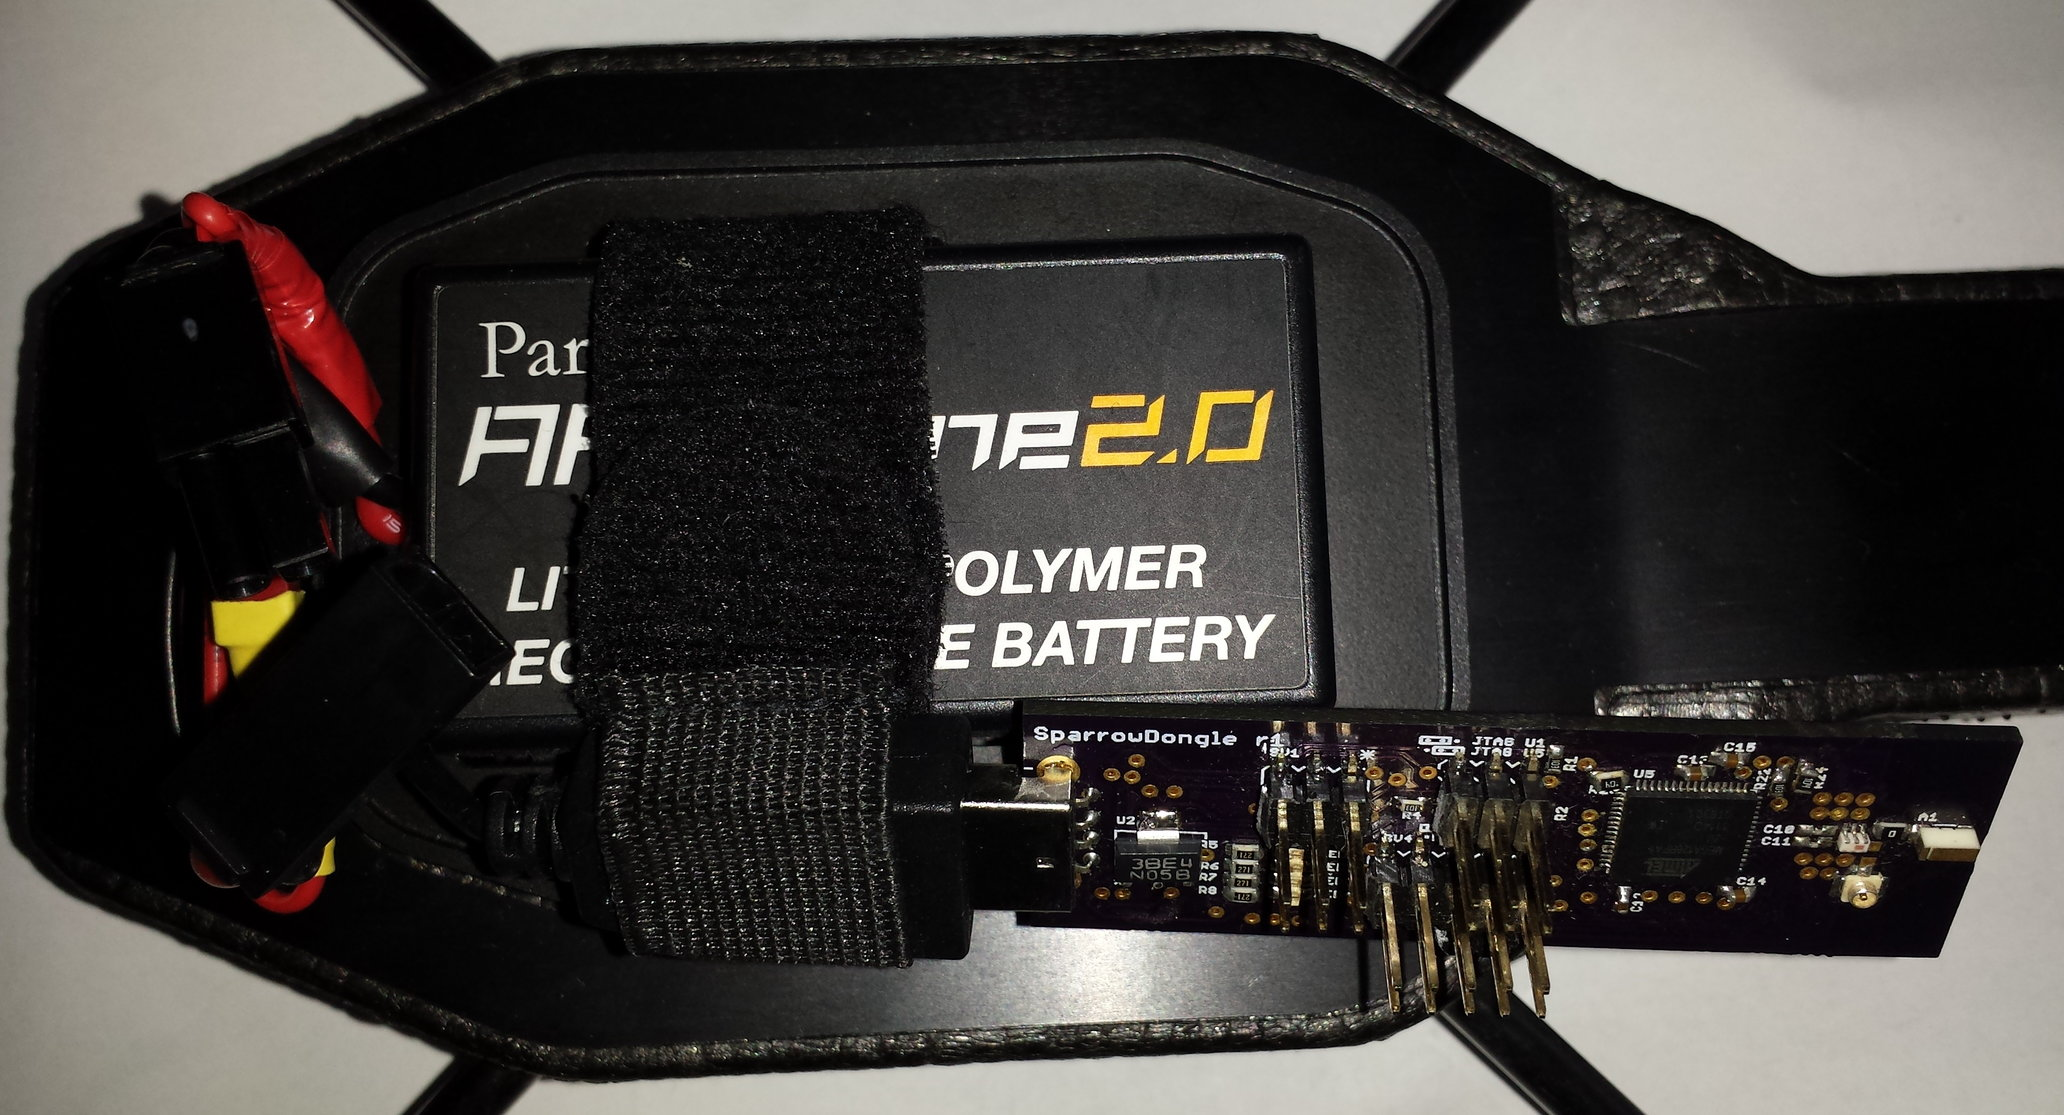
\includegraphics[width=0.45\textwidth]{img/dronedongle.jpg} \caption{SparrowDongle connected to AR Parrot Drone 2.0 } \end{figure}

The hardware components used are the following:
\begin{itemize}

\item a SparrowDongle with two micro controllers: The 8-bit ATMega128RFA1 which has an on-chip 2.4GHz wireless transceiver and the ATMega32U4, both from Atmel.

\item a SparrowV3.2  with an ATMega128RFA1 micro controller 

\item a AR Parrot Drone v2.0

\item a SAMSUNG Galaxy S4 with android 4.4.2, but a laptop or other mobile phones with android/ios can be used for controlling the drone

\end{itemize}

Because of the addition of the SparrowDongle, the drone's polyester hull has had to been carved a little in order to accommodate it.
 

\subsection{Software Implementation}

The parrot drone, with a Linux based operating system, allow the software to be organized in different modules. The modules can be modified individually  to add more features to the system.

The SparrowDongle gateway dumps every data received on the serial. It is always in a listen for data state. When it receives the data, it sends back an ack to let the SparrowV3.2 node know that it can begin sending the entire data to the mobile gateway. 

The SparrowV3.2 node is sending periodically a small data packet to check if a gateway is available. When it receives the ack for the packet it starts sending the stored data to the gateway. The data sent can vary, from sensor readings, to debugging informations in order to check the state of the Wireless Sensor Network.

The data gathered by the gateway is saved into different files the AR Parrot Drone's internal memory. The file also contains informations about the node identification tag and time of the transfer. The data can be accessed at any time by any device connected to the drone's wireless network via FTP.



All the collected data is processed on the drone. It awaits a socket connection in order to start sending informations regarding the state of the connected nodes.

The nodes can be programmed to determine the signal strength of the surrounding nodes. This data is sent to the drone in order to determine the approximate location of the nodes\cite{savarese2001location}.




\section{Results}
\label{sec:results}
\label{chap:results}


\subsection{Power Consumption}

Because the node was designed with low power in mind, we can obtain a very low deep sleep power
consumption of 5uW. This means that we can use a small solar panel together with a
small capacitor to act as the main power supply.

For example, if a 1F capacitor is use with the voltage ranging from 3v3 to 2v1 for complete
discharge, the equivalent battery capacity would be

$$ \frac{F * (Vi - Vf)}{t} = \frac{1F * (3.3V - 2.1V)}{3600s} = 0.333mAh$$

The node is equipped with a DC/DC converter with can bring substantial power savings, depending on
the voltage of the power supply. A LDO wastes a lot off energy as the delta between the
voltages increases, were as DC/DC works best when the delta increases, or putting it simple, if an
LDO ouputs 1v8 and a chip consumes 5mA, the input current is almost the sam 5mA regardless of the
input voltage. So event though the chip consumes 9mW, the total power consumed is actually 25mW. If
in the same situation, a DC/DC with a 90\% efficiency is used, then the input current would be :
$$Iin = \frac{Iout * Vout}{Vin*Efficiency} = \frac{5mA * 1.8V*100}{5v*90}= 2mA$$


we can ignore the quiescent current because it is very small, around 360nA. The total power
consumption in this case is 10mW for an output power of 9mW compared with the LDO which consume
25mW in order to output just 9mW, a 250\% difference between them.

In real world situation, when a battery or a capacitor is used, the difference between them is
smaller. We will present two cases, in order to better understand the influence of higher
voltage supply.

The minimum voltage will be 2v1 for DC/DC and 1v9 for LDO. The current consumption of the chip is
5.5mA, and a capacitor of 1F.

Case 1: Capacitor charged to 3v3.

$$T_{LDO} = \frac{C * (V_i - V_f)}{I}=\frac{1F * (3.3V - 1.9V)}{5.5mA} = 254.45s $$

$$E_i = \frac{C*V_i^2}{2} = \frac{1f*3.3v^2}{2} =5.445J$$
$$E_f = \frac{C*V_f^2}{2} = \frac{1f*2.1v^2}{2} =2.205J$$
$$E = E_i - E_f = 3.24J$$
$$P = V*I*E_{fficiency }= \frac{1.8V * 5.5mA * 90}{100} = 11mW$$
$$T_{DC} = \frac{E}{P} = \frac{3.24J}{11mW} =294.54S $$

$$Advantage = \frac{T_{DC} - T_{LDO}}{T_{LDO}} = \frac{294.54s - 254.45s}{254.45s} = 15.7\%$$

Case 2: Capacitor charged to 5v.

$$T_{LDO} = \frac{C * (V_i - V_f)}{I}=\frac{1F * (5V - 1.9V)}{5.5mA} = 527.27s $$

$$E_i = \frac{C*V_i^2}{2} = \frac{1f*5v^2}{2} =12.5J$$
$$E = E_i - E_f = 10.295J$$
$$T_{DC} = \frac{E}{P} = \frac{3.24J}{11mW} =935.91S $$

$$Advantage = \frac{T_{DC} - T_{LDO}}{T_{LDO}} = \frac{935.91s - 527.27s}{527.27s} = 77.5\%$$

At 3.3V the advantage is not that big, but at 5V we nearly double the battery life. Using a LIPO
battery which does not discharge as linearly as the capacitor, will furthermore increase the
advantage of the DC/DC.

In real world testing, we charged a 1F capacitor up to 3v3 and let it discharge by transmitting data every second. Even though the software was not
optimized for low power, the node managed to run for 8 hours before the capacitor was completely
discharged with translates to an average power consumption for almost 112uW.


\subsection{Software}

The software is open source and can it is compatible with Arduino 1.6.x, latest iteration to date,
May 2016. It was tested using Windows 8.1, but it should be fully compatible with other operating systems as well.

The node has on board native USB which allows for code upload and also serial interface over CDC
useful for debugging and also for versatility, because the same node can be configured as gateway or
as leaf.


\section{Future work}
\label{sec:future}
\label{chap:future}

The versatility of the platform makes it ideal to be deployed in a wide range of applications, especially those of which environment is dynamic.

For instance, some possible applications in which the drone can be deployed are  \cite{arampatzis2005survey}:

 \begin{itemize} 

\item  Autonomous collection of data data by adding a gps receiver to the drone and setting a path of way points to follow

\item Debugging a wireless sensor network by checking which node is working, the connection logs and the physical state of the device

\item Search and rescue operations, especially when going skiing in a avalanche prone environment by wearing a wireless sensor. 

\item Creating a small wireless sensor network for a limited time with small costs and large battery life

\item Treasure hunt where the sensors can hold the clues that lead to the location of the treasure

 
\end{itemize}



\section{Conclusion}
\label{sec:conclusion}
The platform is very easy to use, the only requirement is knowing how to use Arduino Studio, and
even then that can be learn easily. The possibility to select desired voltage and to add hardware on
the fly opens new possibilities and decreases the time needed for an application to be developed.





\bibliographystyle{abbrv}
\bibliography{roedunet-gateway}

\end{document}
